\documentclass[conference]{IEEEtran}
\IEEEoverridecommandlockouts
% The preceding line is only needed to identify funding in the first footnote. If that is unneeded, please comment it out.
\usepackage{cite}


\usepackage{amsmath,amssymb,amsfonts}
\usepackage{algorithmic}
\usepackage{graphicx}
\usepackage{textcomp}
\usepackage{xcolor}
\usepackage{url}
\def\BibTeX{{\rm B\kern-.05em{\sc i\kern-.025em b}\kern-.08em
    T\kern-.1667em\lower.7ex\hbox{E}\kern-.125emX}}
\begin{document}

\title{VIDEO STITCHING WITH SMALL OVERLAP\\
%{\footnotesize \textsuperscript{*}Note: Sub-titles are not captured in Xplore and
%should not be used}
%\thanks{Identify applicable funding agency here. If none, delete this.}
}

\author{\IEEEauthorblockN{1\textsuperscript{st} Chaoyu Xie}
\IEEEauthorblockA{\textit{University of Science and Technology of China} \\
%\textit{name of organization (of Aff.)}\\
Anhui, China \\
xcy12345@mail.ustc.edu.cn}
\and
\IEEEauthorblockN{2\textsuperscript{nd} Xuejin Chen}
\IEEEauthorblockA{\textit{University of Science and Technology of China} \\
%\textit{name of organization (of Aff.)}\\
Anhui, China \\
xjchen99@ustc.edu.cn}
%\and
%\IEEEauthorblockN{3\textsuperscript{rd} Given Name Surname}
%\IEEEauthorblockA{\textit{dept. name of organization (of Aff.)} \\
%\textit{name of organization (of Aff.)}\\
%City, Country \\
%email address}
%\and
%\IEEEauthorblockN{4\textsuperscript{th} Given Name Surname}
%\IEEEauthorblockA{\textit{dept. name of organization (of Aff.)} \\
%\textit{name of organization (of Aff.)}\\
%City, Country \\
%email address}
%\and
%\IEEEauthorblockN{5\textsuperscript{th} Given Name Surname}
%\IEEEauthorblockA{\textit{dept. name of organization (of Aff.)} \\
%\textit{name of organization (of Aff.)}\\
%City, Country \\
%email address}
%\and
%\IEEEauthorblockN{6\textsuperscript{th} Given Name Surname}
%\IEEEauthorblockA{\textit{dept. name of organization (of Aff.)} \\
%\textit{name of organization (of Aff.)}\\
%City, Country \\
%email address}
}

\maketitle

\begin{abstract}
Video stitching remains a challenging problem in computer vision. In this paper, we propose a novel method to stitch multiple videos which have a small overlapped region.
The algorithm consists of three steps: (1) calibrating the camera and project the video frame into spherical coordinates. (2) detecting the edges of each projected frame 
and calculate homegraphy matrix in each grid. (3) updating seam and stitch the origin video to produce a panoramic video. The proposed method has proven to be
more robust on small overlapped region. Experimental results show that our approach achieves better panoramic videos than state-of-the-art ones.
\end{abstract}

\begin{IEEEkeywords}
Video stitching, panorama, overlap, edge detection
\end{IEEEkeywords}

\section{Introduction}
\label{sec:intro}

Video stitching is the process to merge several videos
including overlapped regions into a panoramic video. The
holy goal of video stitching is to acquire a large view video
that looks as natural as possible. As a result of the widespread
use in security monitoring, virtual reality and medical image
analysis, video stitching has become a hot topic in recent years.

However, in previous video stitching systems \cite{zheng2008stitching, guo2016joint, Jiang_2015_CVPR_Workshops, nie2018dynamic},
cameras used to capture multiple videos usually have large overlap, which can be easily handled.
Under this circumstance, there are lots of commercial softwares such as VideoStitch Studio \cite{videostitching}, AutoPano \cite{autopano},
compute a stitching model, which is usually a 2D transformation,
according to the relative position and angle between two cameras. 
When the overlap between cameras is very small, these methods and softwares can
not work as good as we expected.

In this paper, we try to solve the problem of stitching videos which have small overlap. 
For example, a typical scenario we envision is: six cameras fixed on 
a tripod. Fig. \ref{fig:equipment} shows our device and the origin data. Although the field of view (FOV) of the cameras is very large, the overlap between the 
cameras is still small. Stitching such six videos is very challenging due to two
major reasons: (1) the captured videos have small overlap that the feature points can not be matched correctly 
and (2) the structure of the building in the panoramic video could have ghost.
To deal with this problem, we proposed a new method which can handle the problem that we have listed above.
Different from the period work \cite{Jiang_2015_CVPR_Workshops}, we mainly focus on video stitching which has a small overlapping area.
Our algorithm first calculate the parameters of the cameras, and then project
the videos into sphere. We extract the edge of each video, and according to the edge we mesh these video into grids frame by frame.
And calculating the homegraphy matrix of each gird. Finally, we update seam and produce a panoramic video.
Fig. \ref{fig:res} shows the video stitching process presented in this paper.

\begin{figure}[t]
\centering
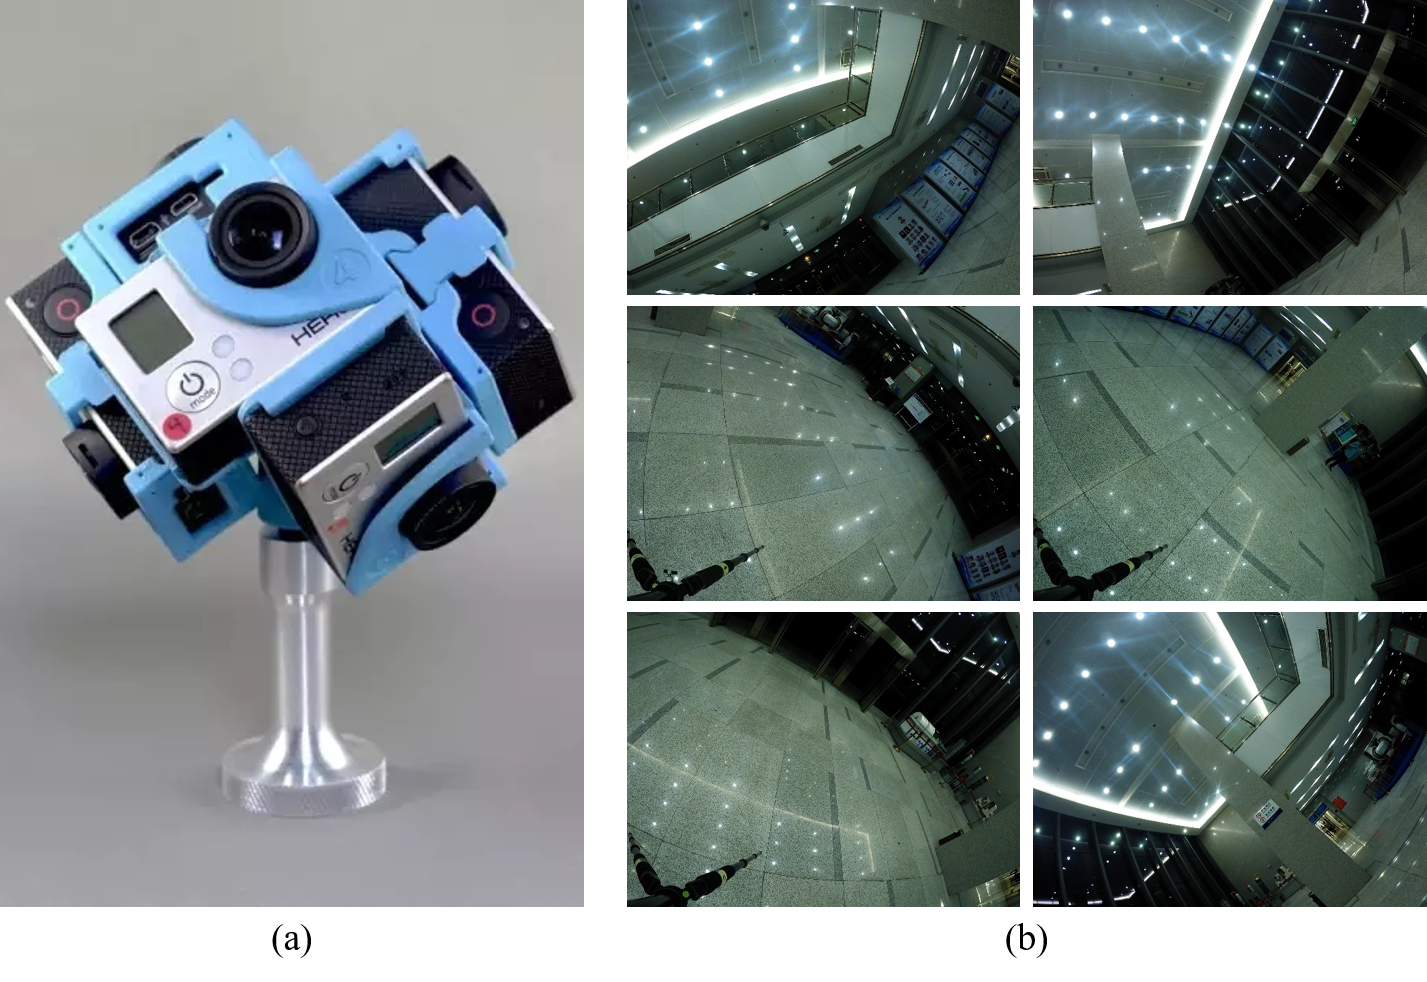
\includegraphics[scale=0.36]{picture34.png}
\caption{The device we use in this paper and the video example. (a) shows the six cameras fixed on a cube, (b) shows the example of videos captured by our devices.}
\label{fig:equipment}
\end{figure}

\begin{figure*}
\centering
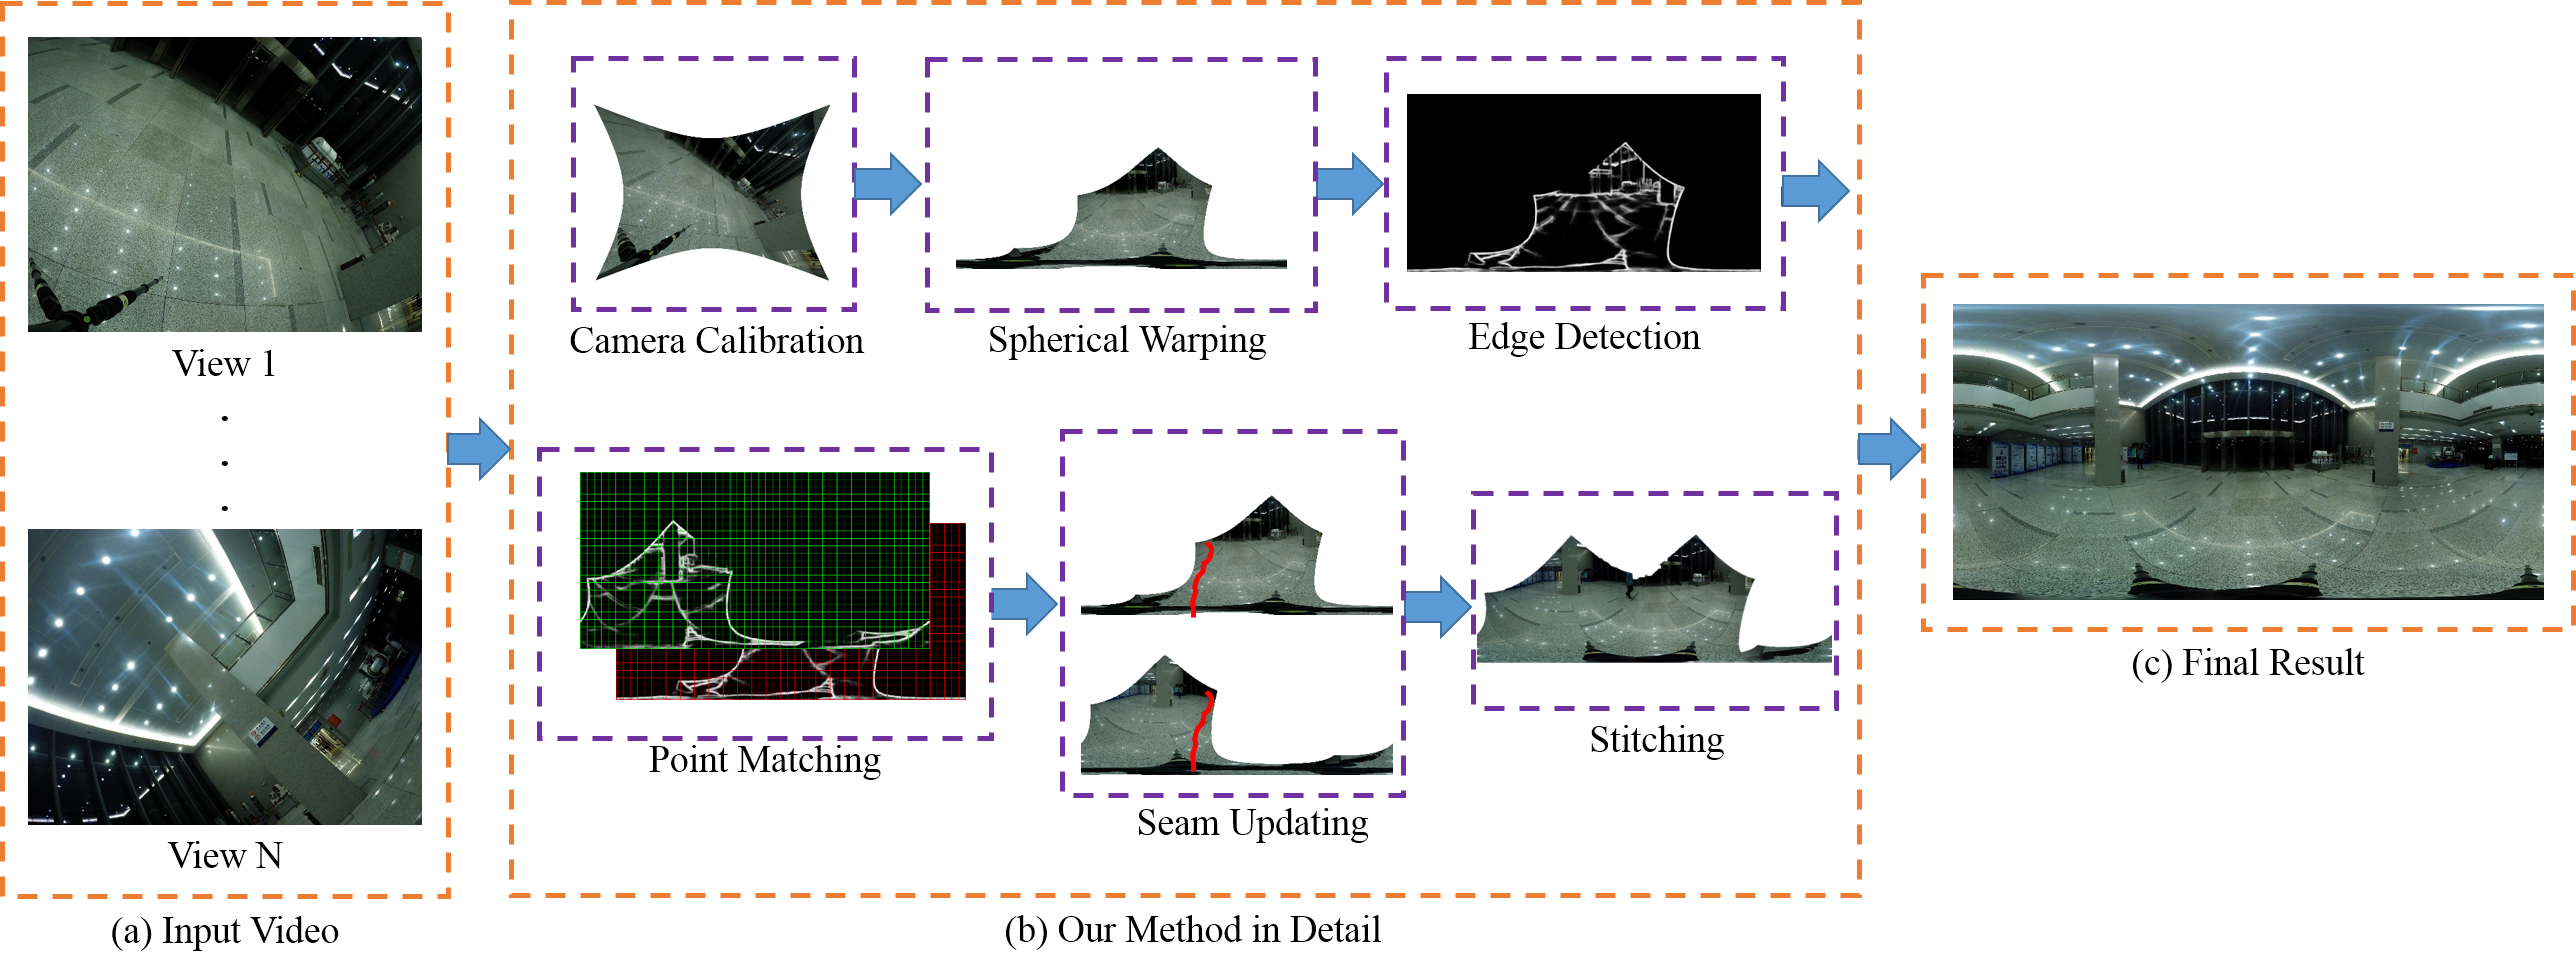
\includegraphics[scale=0.26]{picture39.png}
\caption{The pipeline of our video stitching algorithm. First, we pre-process the video data, such as calibrate the camera
and project the video frame into spherical coordinates. Second, we detect the edge of each projected frame and re-calculate
homegraphy matrix in every grid. Third, update seam and stitch the videos to produce a panoramic video.}
\label{fig:res}
\end{figure*}

\section{Related work}
\label{sec:related}

In this section, we briefly review the most related works in image stitching and video stitching.\\
{\bf Image Stitching}: Image stitching is a well-studied, yet still active research 
area in \cite{paragios2006handbook, brown2007automatic,hartley2003multiple,lin2011smoothly, chang2014shape, zaragoza2013projective,lin2015adaptive,zhang2014parallax, gao2013seam, agarwala2004interactive}. 
Early methods adopted a single homegraphy to align images. The single homegraphy 
is valid only when the camera only rotates around its optical center or the scene captured 
is planar \cite{hartley2003multiple}. When there is parallax between the images, 
artifacts such as structure distortion and 
ghost occur. In general, there are two kinds of stitching strategies: 
warp-based \cite{lin2011smoothly, chang2014shape, zaragoza2013projective} and 
seam-driven \cite{zhang2014parallax, gao2013seam, agarwala2004interactive}. In the warp-based category, 
Gao \textit{et al.} proposed to use two homographies for image stitching 
when the scene could be modeled roughly by two planes (ground plane and distant plane) \cite{gao2011constructing}.
Zaragoza \textit{et al.} proposed an as-projective-as-possible (APAP) mesh deformation that warps
images by following a global projective transformation and allows local non-projective 
deviations \cite{zaragoza2013projective}.
Chang \textit{et al.} proposed a shape-preserving half-projective (SPHP) method
to correct distortions in non-overlapping regions \cite{chang2014shape}. 
Lin \textit{et al.} proposed Adaptive As-Natural-As-Possible (AANAP) 
which based on APAP but computes the warpping fully automated \cite{lin2015adaptive}.
In the seam-driven category, Agarwala \textit{et al.}
proposed photomontage that composites a photograph by
cutting and stitching multiple photographes seamlessly \cite{agarwala2004interactive},
while Zhang and Liu looked for a homography that leads to a
minimum energy seam to stitch large-parallax images \cite{zhang2014parallax}.
In addition, several freewares and commercial softwares are available for performing image stitching.
AutoStitch, Microsoft’s Image Compositing Editor, and Adobe's Photoshop CS6 mosaicing feature.\\
{\bf Video Stitching}: Compared to image stitching, video stitching received much less attention.
Different approaches have been proposed for different camera settings. In general, these can be divided into two categories: 
fixed cameras \cite{zheng2008stitching, he2010panoramic, Jiang_2015_CVPR_Workshops, perazzi2015panoramic, li2015efficient} 
and moving cameras \cite{lin2016seamless, guo2016joint, nie2018dynamic}. In the fixed cameras category, 
Zheng \textit{et al.} stitched the videos frame by frame just like image stitching \cite{zheng2008stitching}.
Jiang \textit{et al.} proposed a method according to the former frame to stitch the video  \cite{Jiang_2015_CVPR_Workshops}.
In the moving cameras category, 
Lin \textit{et al.} proposed a method which is for independently moved mobile devices.
They recovered the 3D camera paths and a sparse set of 3D scene points to stitching videos \cite{lin2016seamless}.
Guo \textit{et al.} estimated both inter
motions and intra motions, then estimate the camera path, and finally stitching them together \cite{guo2016joint}.
Nie \textit{et al.} which was similarly to \cite{guo2016joint} but could distinguish between right
and false matches \cite{nie2018dynamic}. All these works have one thing in common, that
is the overlap between the cameras is large. Under this circumstance, stitching 
become much more easier. However, in this paper, we will stitch videos
which have a very small overlap between the cameras.

\section{OUR METHOD}
\label{sec:ourmethod}

Fig. \ref{fig:res} shows the pipeline of our video stitching algorithm.
The first step of our algorithm is calculating the parameters of the cameras, and projecting the origin video into a spherical coordinate system frame by frame, 
see details in Sec. \ref{ssec:Pre-prepared}. The second step is to extract the edge on every frame and mesh the frame into grid and calculate homegraphy matrix in each grid. 
Then matching the points in overlapped region which is described in Sec. \ref{ssec:edge-detection}. 
The third step is to stitch them into a panoramic video according to the spatial-temporal information, as described in Sec \ref{ssec:stitching}.

\subsection{Pre-process For Video Stitching}
\label{ssec:Pre-prepared}
Pre-process for video stitching composes of two parts, the one is calculating the parameters of the cameras, the other is to project the video into a new coordinate
system. The parameters of a camera consist intrinsics and extrinsics. 
%Because the camera is fixed on a tripod, we can easily calculate the extrinsics of the cameras. 
According to \cite{zhang2000flexible}, we calculate the intrinsics and extrinsics of the cameras.
Then video can be projected into spherical coordinate system.
%Denote the origin video as $F_g$, and the projected video as $F$, 
Let $\textbf{x} = [x \ y]^T$ be the point of projected frame $F$ and $\hat{\textbf{x}'} = [\hat{x}' \ \hat{y}']^T$ be the point of  calibrated frame $F_g$.
%And denote $\hat{\textbf{x}}' = [\hat{x}' \ \hat{y}' \ \hat{z}']^T$ to be the spherical coordinates. Because the frames should be projected into the same coordinate system, the $\hat{\textbf{x}}'$
%should be multiplied extrinsics matrix. 
The relationship between $F$ and $F_g$ can be described as following equation:
\begin{equation}
\begin{aligned}
x'=sinxcosy, y'&=siny, z'=cosxsiny\\
\left[ \begin{array}{l}{\hat{x}} \\ {\hat{y}} \\ {\hat{z}}\end{array}\right]&=\textbf{R} \left[ \begin{array}{l}{x^{\prime}} \\ {y^{\prime}} \\ {z^{\prime}}\end{array}\right]\\
\hat{x}'&=f\frac{\hat{x}}{\hat{z}}+x_c\\
\hat{y}'&=f\frac{\hat{y}}{\hat{z}}+y_c
\end{aligned}
\end{equation}
where $\textbf{R}$ stands for the extrinsics matrix. $x_c$ and $y_c$ stands for the center of $F$.
Fig \ref{fig:ori_cal_pro} shows the origin frame, 
calibrated frame and projected frame. 

\begin{figure}[t]
\centering
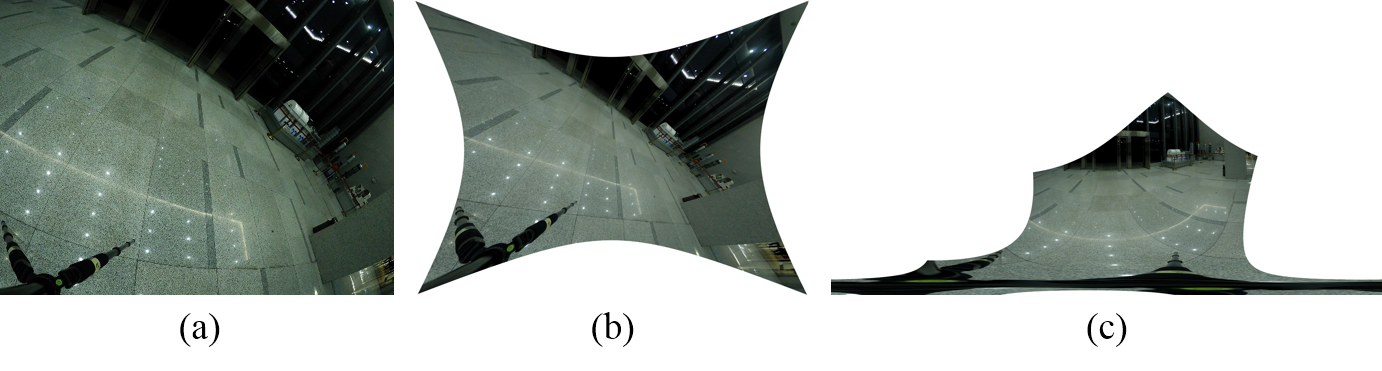
\includegraphics[scale=0.23]{picture40.png}
\caption{(a) shows the origin frame, (b) depicts the calibrated frame calculated from (a), (c) illustrates the projected frame calculated from (b).}
\label{fig:ori_cal_pro}
\end{figure}
\subsection{Edge Detection and Points Matching}
\label{ssec:edge-detection}
%After we got the projected frame, we can 
Because the overlapped region is small, we can not match the feature points correctly. Although we got the projected frame, we still can not 
match the feature points correctly because of the complicated scenes we captured. Under this circumstance, we propose to detect its edge and then match points according to the edge.
We use a matured method which is called holistically-nested edge detection (HED) \cite{xie2015holistically}. After we got the edge of each frame, we mesh every frame into $m \times n$
girds. In the overlapped region, it can be easily to match the points after detecting its edge. Let $\textbf{a} = [i \ j]^T$ and $\textbf{a}' = [i' \ j']^T$ be matching points
across overlapping frames $F_l$ and $F_r$. A projective warp or homegraphy aims to map $\textbf{a}$ to $\textbf{a}'$ following the relation:
\begin{equation}
\widetilde{\textbf{a}}'=\textbf{H}\widetilde{\textbf{a}}
\end{equation}
where $\widetilde{\textbf{a}}$ is $\textbf{a}$ in homogeneous coordinates, and $\textbf{H}\in\mathbb{R}^{3 \times 3}$ defines the homegraphy. In the overlapped region,
we can detect its nearest neighbor point as its matching point. Then calculate the homegraphy matrix in each grid. According to the matrix, the points can be projected to the correct region.
However, there maybe some grids that have no points, we can calculate the homegraphy matrix according to its four neighbor grids. Let $\textbf{H}_i$ be the homegraphy matrix in grid $i$.
The $\textbf{H}_{i}$ can be calculated as following if there is no points are detected:
\begin{equation}
\textbf{H}_{i} = \frac{1}{4}\left(\textbf{H}_{il}+\textbf{H}_{ir}+\textbf{H}_{iu}+\textbf{H}_{id}\right)
\end{equation} 
where $\textbf{H}_{il}$, 
$\textbf{H}_{ir}$, 
$\textbf{H}_{iu}$, 
$\textbf{H}_{id}$ 
denote four neighbor homegraphy matrices of grid 
$i$.
Fig. \ref{fig:p8} illustrates the method we proposed.
\begin{figure}[!htpb]
\centering
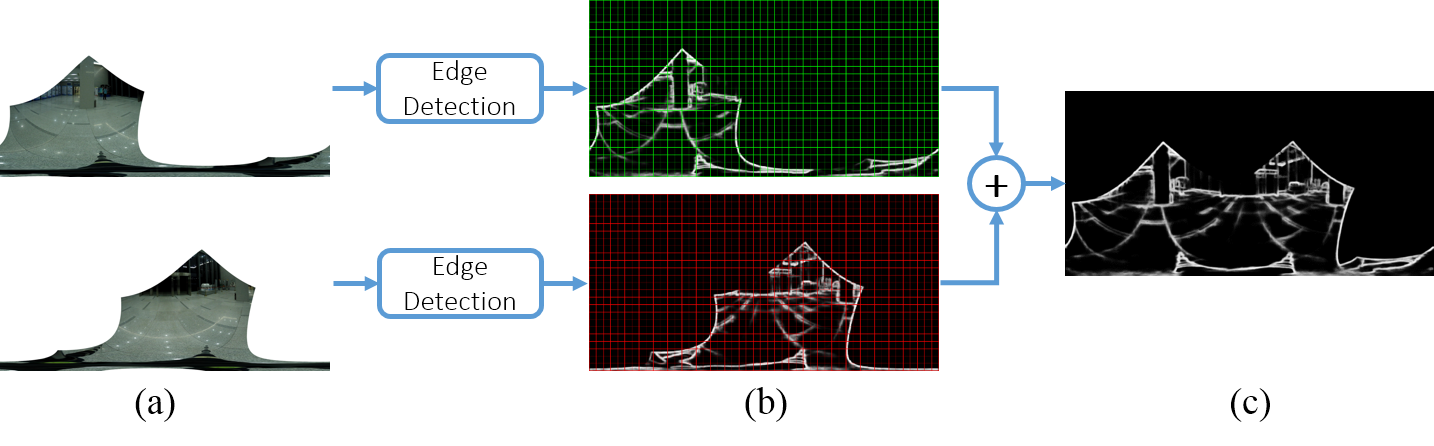
\includegraphics[scale=0.22]{picture41.png}
\caption{First the projected frame will be detected by HED \cite{xie2015holistically}, and the edge detected frame mesh into $m \times n$ grids, then the overlapped region calculated its homegraphy matrix in grid $i$.
Finally output a new frame combined with two edge detected frames. (a) depicts the projected frame, (b) shows the grids in each frames, (c) shows the new edge produced by (b).}
\label{fig:p8}
\end{figure}

\subsection{Seam Updating and Stitching}
\label{ssec:stitching}

%After we got the edge frame, we can 
Using the method we proposed in Sec. \ref{ssec:Pre-prepared} and Sec. \ref{ssec:edge-detection}, the structure of buildings in the video can be preserved. However, when there is a moving object
through the overlapped region, there may exist ghosts in the panoramic video. 
%To obtain final panoramic video, we transform input videos by the estimated stitching and stabilization variables. 
In the overlapping region, background is stitched using the method we proposed in Sec. \ref{ssec:edge-detection}, but not surprisingly, 
foreground objects have ghost artifacts, especially when there is an object moving through the overlapped region. To stitch the
two videos seamlessly, we adopt the overlaying strategy as in \cite{he2016parallax}. Firstly, we search a seam in the overlapping region according to our homegraphy matrices which was calculated in \ref{ssec:edge-detection}.
Secondly, use $\widetilde{g}_{i0}$ as the original gradient of pixel $p_i$ in the present seam, and use $\widetilde{g}_{it}$ as the gradient of pixel $p_i$ in time $t$. To calculate whether the gradient
of pixels have a big change, we use the following rule:
$$
\textit{C}_{t}=\{p_{i}|\frac{\widetilde{g}_{it}-\widetilde{g}_{i0}}{\widetilde{g}_{i0}}>\sigma\}
$$
where $\sigma$ is a const, $\textit{N}_{cd}$ is depended on the total pixel number of the seam. If the total pixel number in $\textit{C}_t$ is bigger than $\textit{N}_{cd}$, we think that there is an object moving through the overlapped region, and then, the seam will be updated.
Finally, to stitch the video well, we use graphcut algorithm \cite{boykov2004experimental} to stitch the frames which have no object moving through the overlapped region. And the others used linear blending method.
Fig \ref{fig:p24} shows the method.
\begin{figure}[h]
\centering
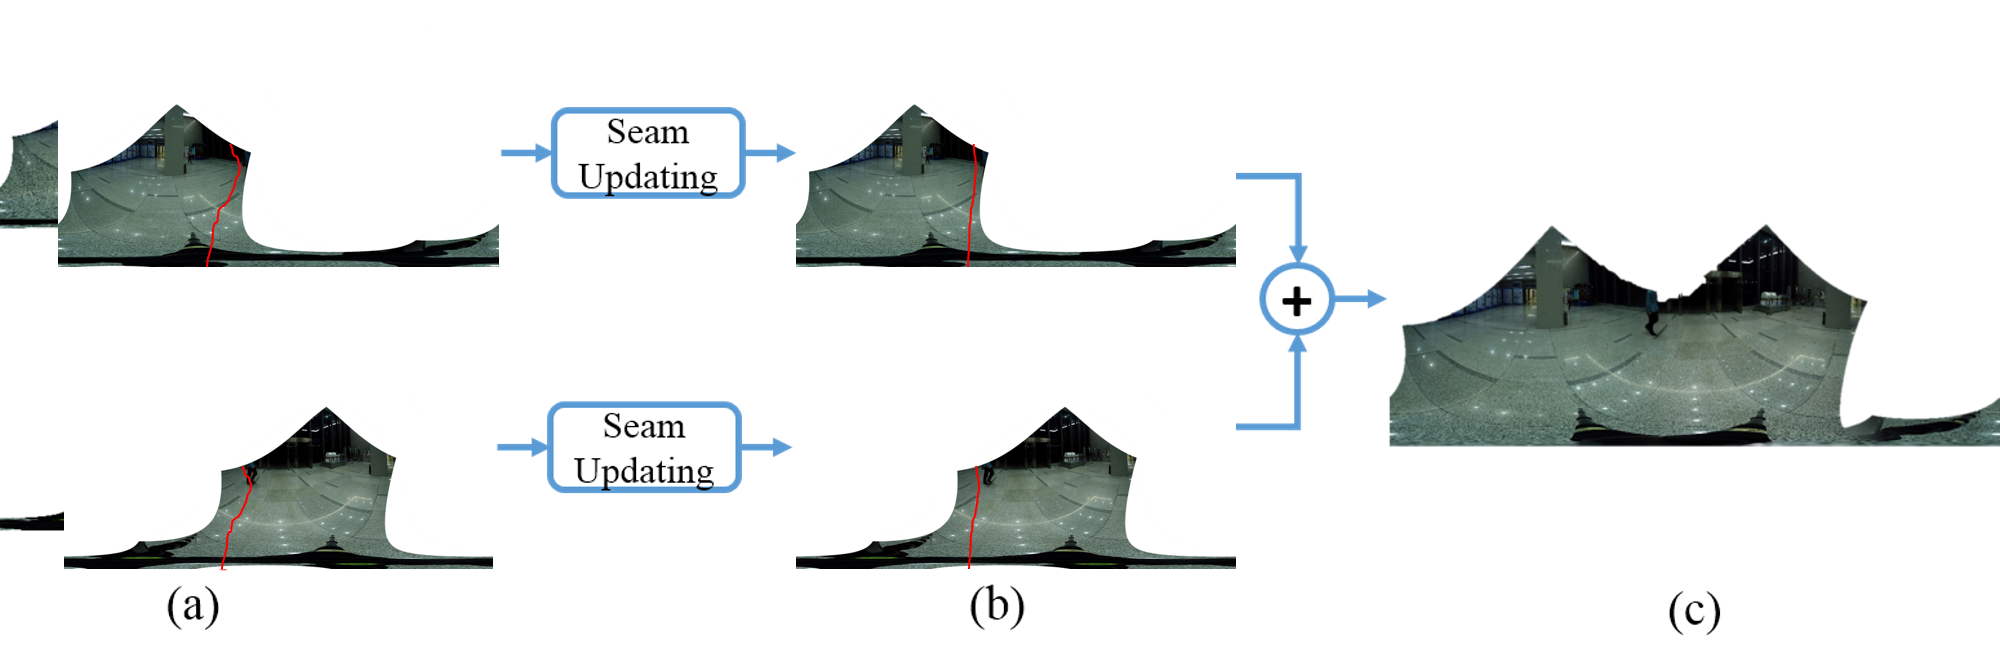
\includegraphics[scale=0.21]{picture43.png}
\caption{Two continuous frames are updated seam according the moving the object. And then stitch them together. (a) shows the origin seam in red line, (b) shows the seam updates 
by algorithm \cite{he2016parallax} in red line,
(c) shows the stitching result.}
\label{fig:p24}
\end{figure}

\section{RESULT}
\label{sec:result}

Since there is no publicly available video stitching benchmark data, we evaluate the proposed method on the 
video which we captured.  The video datasets are captured by six fixed cameras (Gopro Hero4 Black) with different views which are synchronized. 
These videos are both captured by same type cameras and they are 1440p (1920 $\times$ 1440) at 24 fps.
Because the overlapped region is very small, lots of method we listed in Sec. \ref{sec:related} failed to stitch them together.
The compared methods include APAP and commercial software AutoPano. The video data used for APAP method in this paper was after pre-processed. We compare the result as image stitching on each frame firstly.
%Fig. \ref{fig:pic14} shows the result between AutoPano and ours. 
We randomly select one frame on image stitching. Fig. \ref{fig:pic17} shows the result of APAP, AutoPano and ours. 
From Fig. \ref{fig:pic17} we can see the result of APAP 
destroys the structure of building severely, such as the pillar and the light. There are severe ghost around pillar and light.
As for commercial software, it also can not stitch the image well, such as the pillar have ghosts and the structure of light breaks from the middle, 
but our method keeps the structure well, and has less ghost than the others.

For comparison of moving object through overlapped region, we compare the result of APAP, AutoPano and ours. Fig. \ref{fig:pic15} 
illustrates frames where an object are moving in the overlapped region and the background remains still. 
We select three consecutive frames for comparison. In Fig. \ref{fig:pic15}, APAP and AutoPano have severe ghosts around the walking person in the panoramic video. 
The man’s body is distorted in AutoPano method. However, using our proposed method, the man's body is kept well. Fig. ~\ref{fig:more1}, Fig. ~\ref{fig:more2} show more comparison of our method and the others.
\begin{table}[!htpb]
\caption{MOS of three algorithms}
\label{tab1:table1}
\centering
\begin{tabular}{c|c|c|c}
\hline
Method& AutoPano& APAP& Ours\\
\hline
MOS& 6.45& 4.54& \bf{7.43}\\
\hline
\end{tabular}
\end{table}
\begin{figure}[!htpb]
\centering
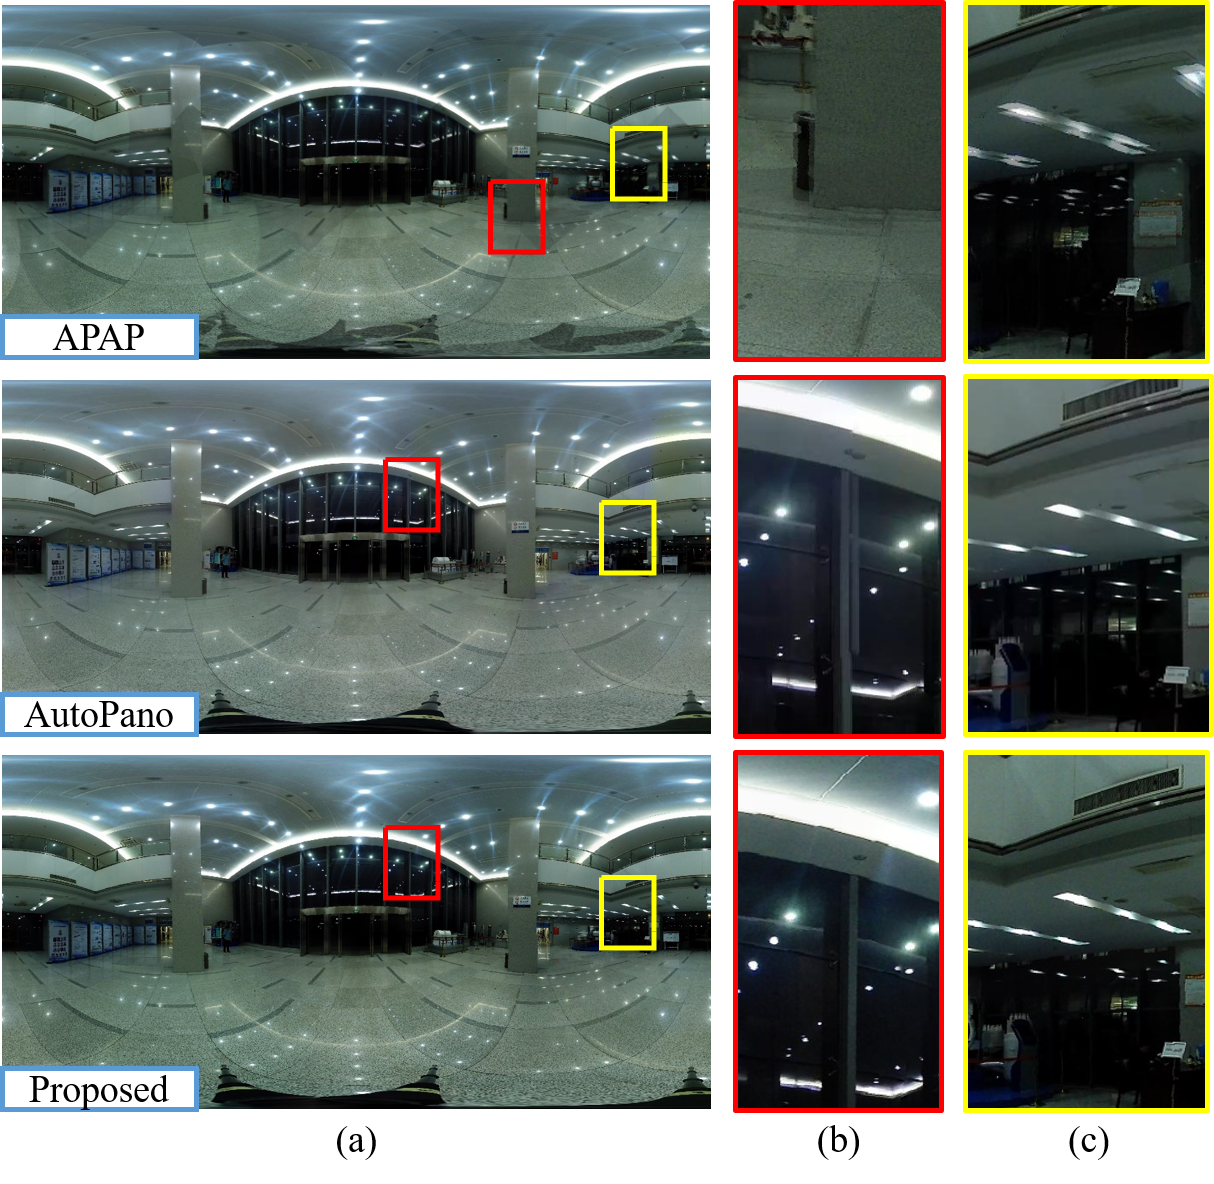
\includegraphics[scale=0.415]{picture35.png}
\caption{Comparisons with APAP, AutoPano and our method. From left to right: (a) one of the stitched frames, (b) enlarged views of local
detail in red box, (c) enlarged views of local detail in yellow box.}
\label{fig:pic17}
\end{figure}
\begin{figure}[!htpb]
\centering
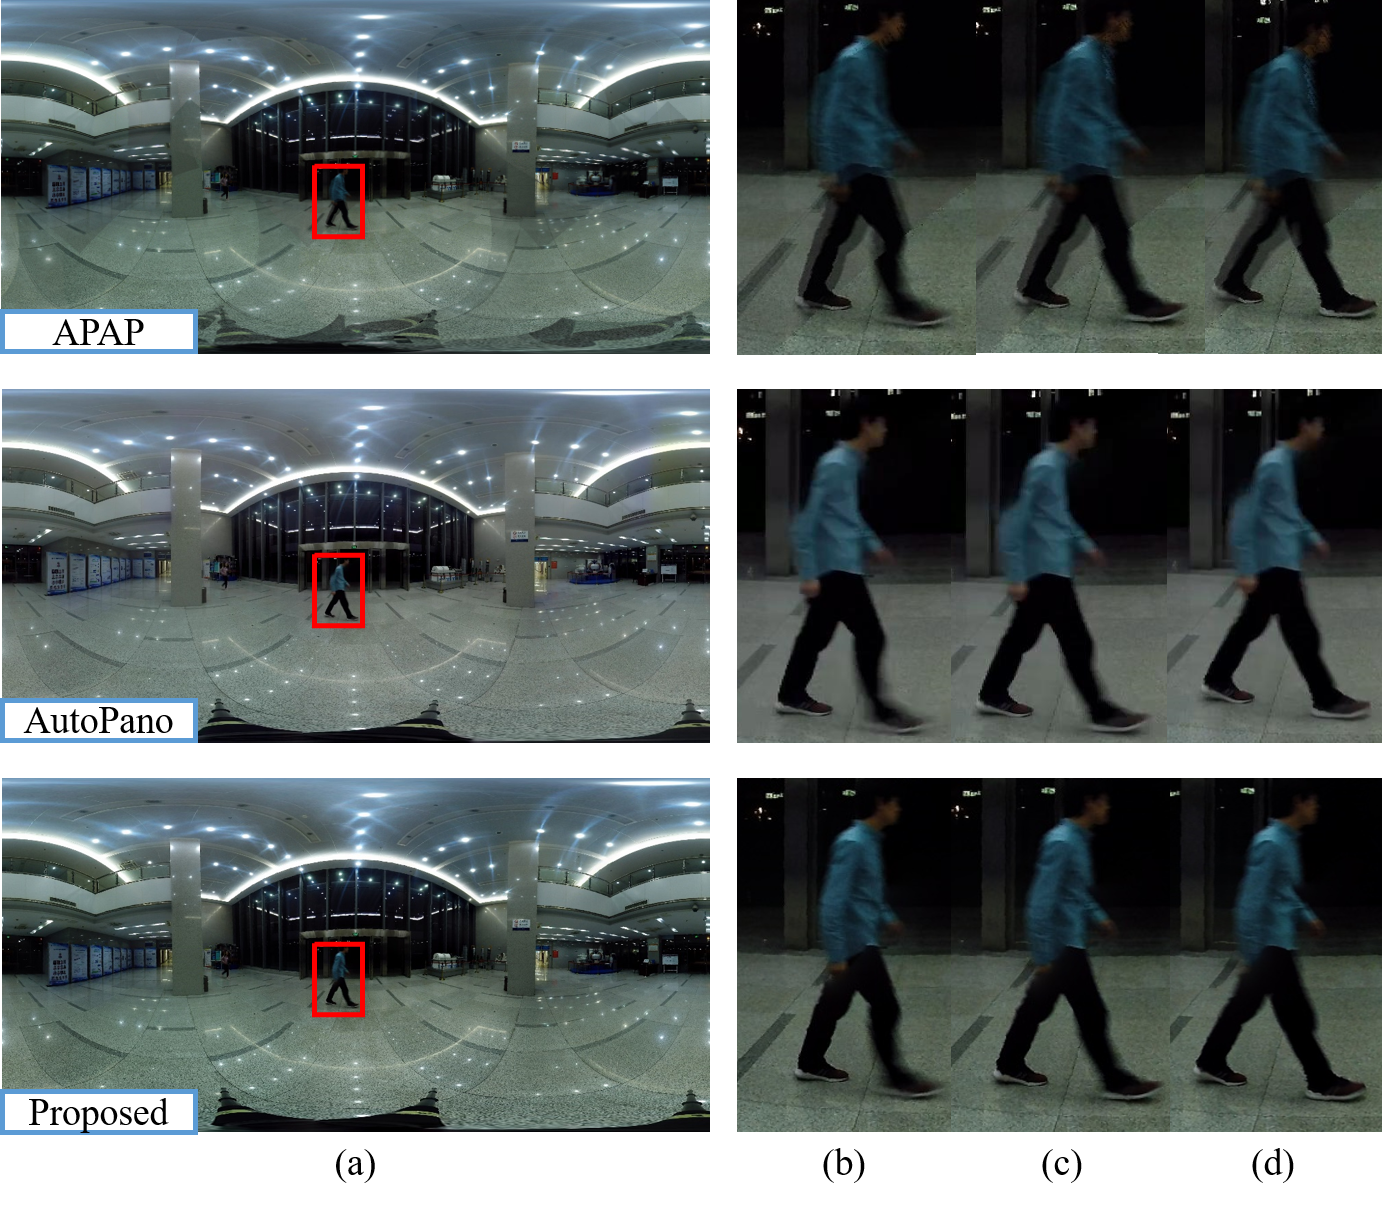
\includegraphics[scale=0.36]{picture36.png}
\caption{Comparisons with APAP, AutoPano and our method when there is an object moving in the overlapped region. From left to right: (a) one of the stitched frames, (b) enlarged views of local
detail in frame $t_1$, (c) enlarged views of local detail in frame $t_2$, (d) enlarged views of local detail in frame $t_3$.}
\label{fig:pic15}
\end{figure}

In order to evaluate the performance of our algorithm, we made a user test interface. The interface shows the results of APAP, AutoPano and our method simultaneously.
We use Mean opinion score (MOS) to evaluate the panoramic video. We use 1-10, 10 integers to represent the quality of the video, 
1 represents the worst quality of the video, 10 represents the best quality of the video, and the method of calculating MOS is as follows:
$$MOS=\frac{\sum^{N}_{n=1}{R_n}}{N}$$
where $N$ stands for the number of people scoring each method and $R_n$ stands for a user's score for each type of video. We take $N=250$ in this experiment.
In the user study, 50 users completed the test according to the rules in which the video groups were random and the video types were random.
And then calculated MOS for each method. Table \ref{tab1:table1} shows the comparison. The MOS of our method is much higher than the others.



\section{CONCLUSION}
\label{sec:conclusion}

In this paper, we proposed a new method to stitch video which have a small overlapped region. We pre-process the video data, such as calibrate the camera and project the video frame into spherical
spherical coordinates. We detect the edge of each projected frame and re-calculate homegraphy matrix in every grid. Using the time domain information to produce a panoramic video. 
Experimental results show that our approach achieves a better panoramic video than state-of-the-art ones. Our algorithm improve image alignment accuracy and reducing artifacts caused by
moving objects. In the future, we would like to speed up our algorithm.

\bibliographystyle{IEEEbib}
\bibliography{refs}
\begin{figure}[!htpb]
\centering
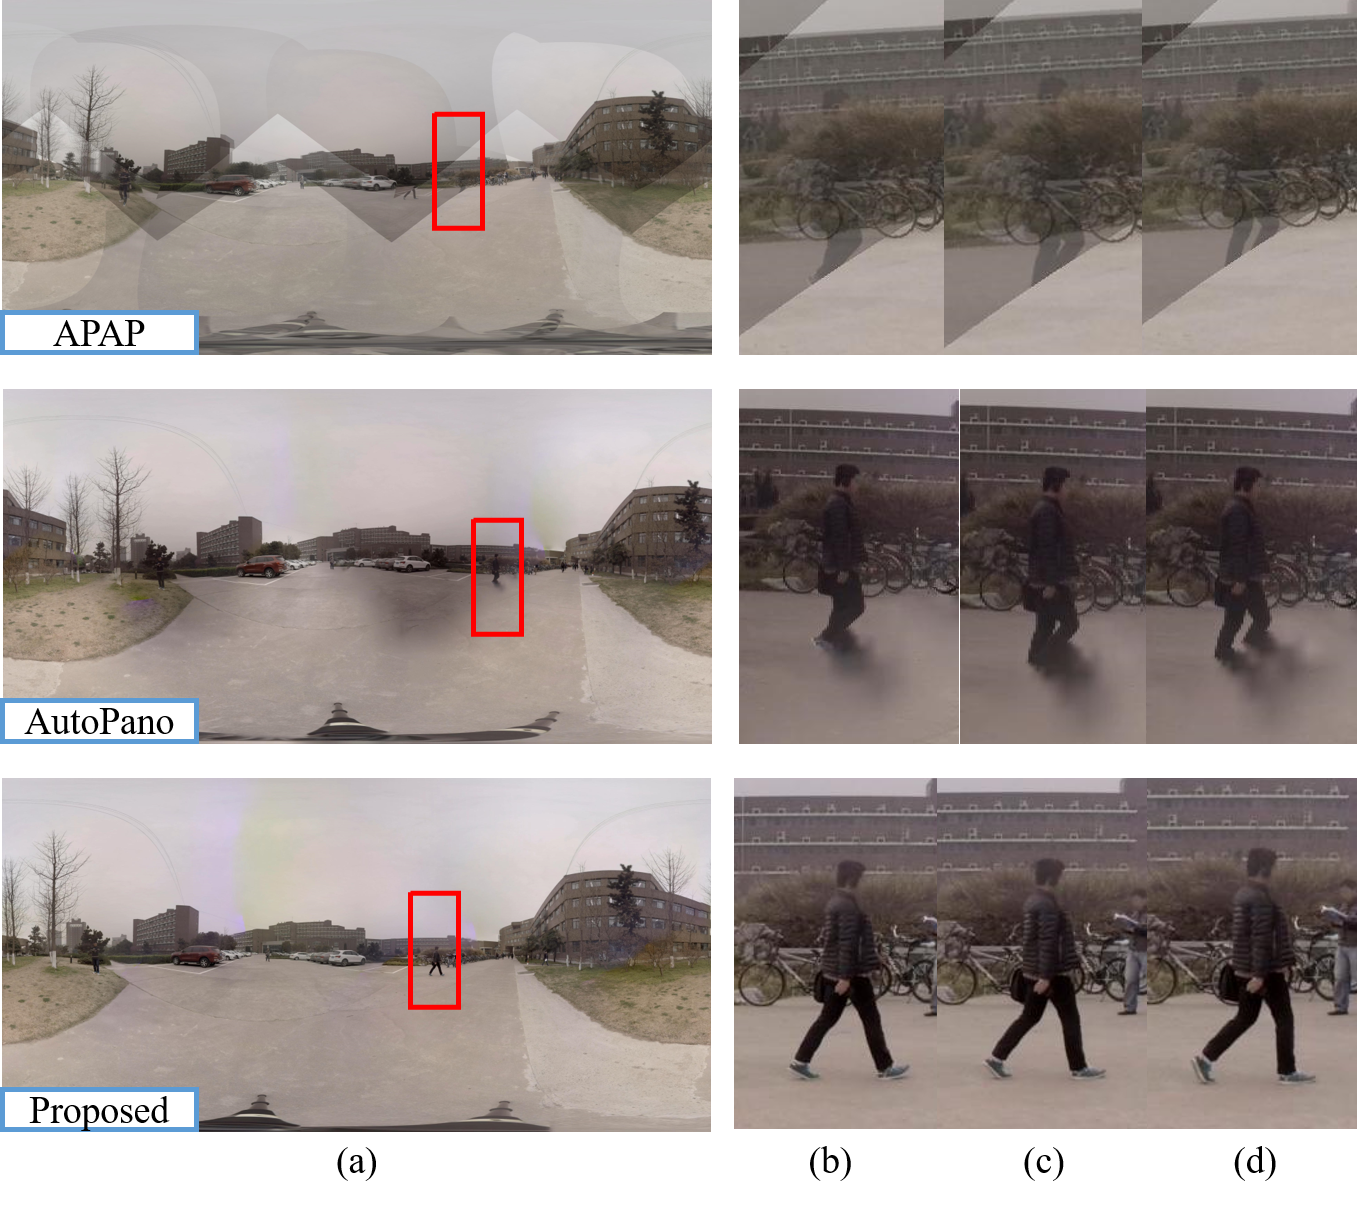
\includegraphics[scale=0.38]{picture37.png}
\caption{Comparisons with APAP, AutoPano and our method when there is an object moving in the overlapped region. From left to right: (a) one of the stitched frames, (b) enlarged views of local
detail in frame $t_1$, (c) enlarged views of local detail in frame $t_2$, (d) enlarged views of local detail in frame $t_3$.}
\label{fig:more1}
\end{figure}
\begin{figure}[!htpb]
\centering
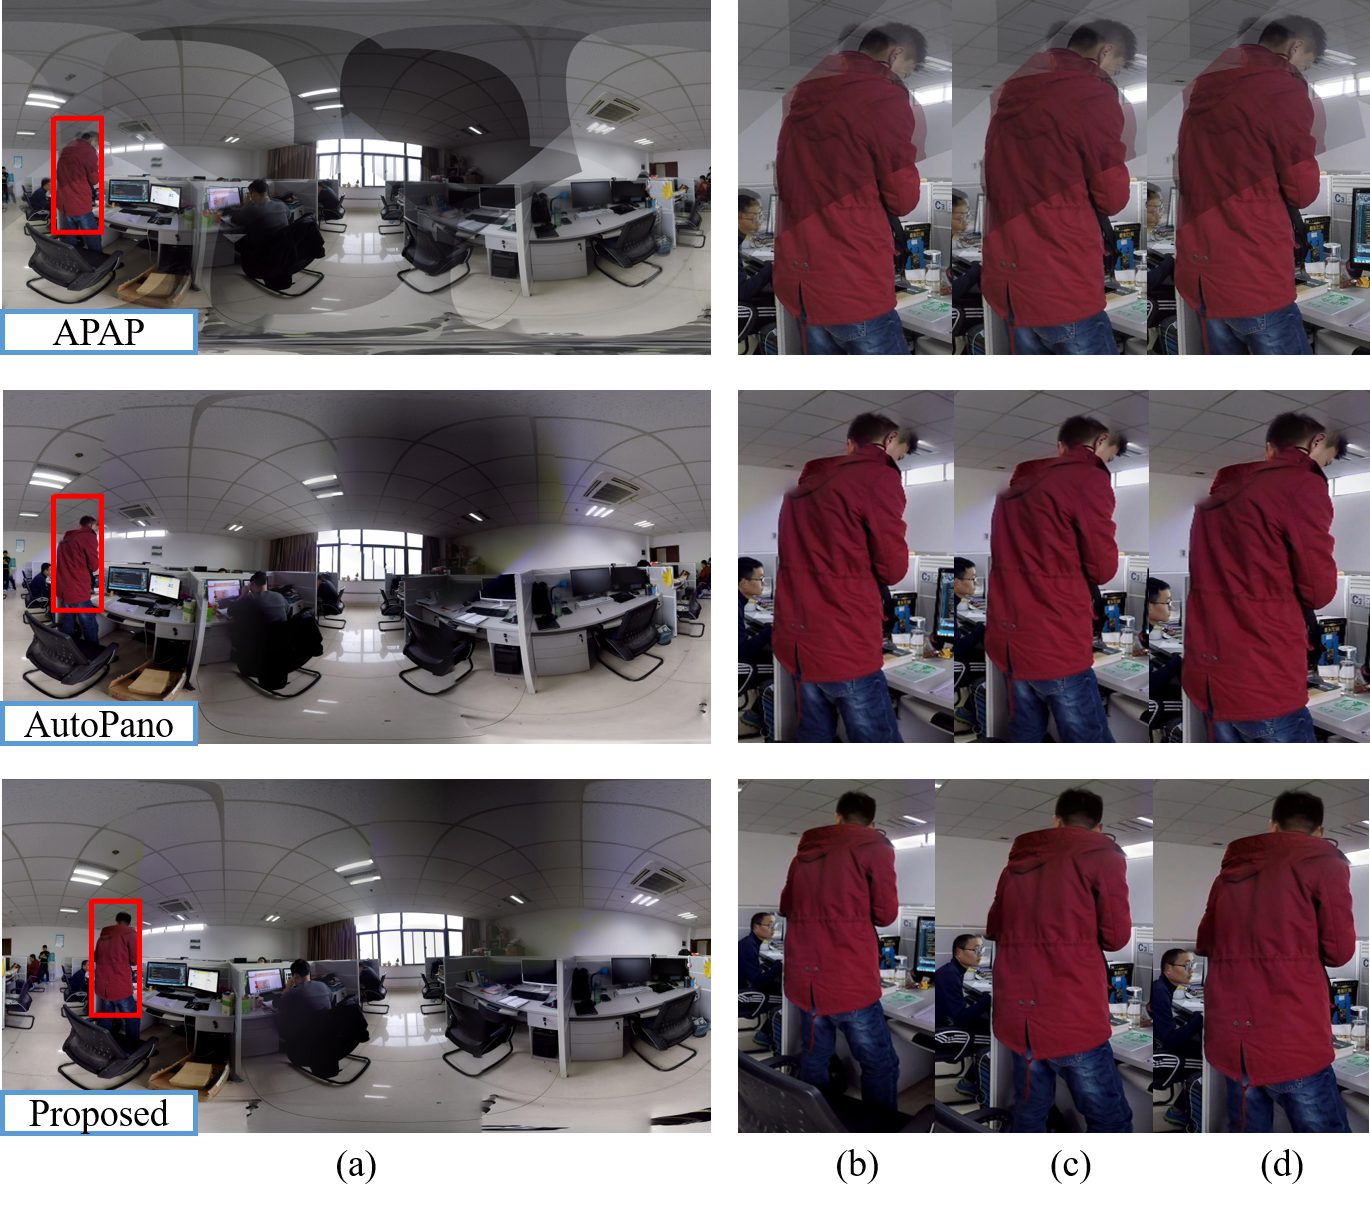
\includegraphics[scale=0.38]{picture38.png}
\caption{Comparisons with APAP, AutoPano and our method when there is an object moving in the overlapped region. From left to right: (a) one of the stitched frames, (b) enlarged views of local
detail in frame $t_1$, (c) enlarged views of local detail in frame $t_2$, (d) enlarged views of local detail in frame $t_3$.}
\label{fig:more2}
\end{figure}
%\section*{References}

%\begin{thebibliography}{00}
%\bibitem{b1} G. Eason, B. Noble, and I. N. Sneddon, ``On certain integrals of Lipschitz-Hankel type involving products of Bessel functions,'' Phil. Trans. Roy. Soc. London, vol. A247, pp. 529--551, April 1955.
%\bibitem{b2} J. Clerk Maxwell, A Treatise on Electricity and Magnetism, 3rd ed., vol. 2. Oxford: Clarendon, 1892, pp.68--73.
%\bibitem{b3} I. S. Jacobs and C. P. Bean, ``Fine particles, thin films and exchange anisotropy,'' in Magnetism, vol. III, G. T. Rado and H. Suhl, Eds. New York: Academic, 1963, pp. 271--350.
%\bibitem{b4} K. Elissa, ``Title of paper if known,'' unpublished.
%\bibitem{b5} R. Nicole, ``Title of paper with only first word capitalized,'' J. Name Stand. Abbrev., in press.
%\bibitem{b6} Y. Yorozu, M. Hirano, K. Oka, and Y. Tagawa, ``Electron spectroscopy studies on magneto-optical media and plastic substrate interface,'' IEEE Transl. J. Magn. Japan, vol. 2, pp. 740--741, August 1987 [Digests 9th Annual Conf. Magnetics Japan, p. 301, 1982].
%\bibitem{b7} M. Young, The Technical Writer's Handbook. Mill Valley, CA: University Science, 1989.
%\end{thebibliography}
%\vspace{12pt}
%\color{red}
%IEEE conference templates contain guidance text for composing and formatting conference papers. Please ensure that all template text is removed from your conference paper prior to submission to the conference. Failure to remove the template text from your paper may result in your paper not being published.

\end{document}
